\section{Machine Learning : metodi e caratteristiche}
\label{ML: metodi e caratteristiche}

In questo capitolo da prima verranno descritti i due approcci principali al ML: l'apprendimento supervisionato(\ref{app_sup}) e non supervisionato (\ref{app_non_sup}). Successivamente verranno presentati due metodi di apprendimento supervisionato, cioè le $\textit{Reti Neurali}$ (\ref{reti neurali}) e gli $\textit{Alberi Decisionali}$ (\ref{alberi decisionali}), ed un metodo di apprendimento non supervisionato, cioè il $\textit{Variational Autoencoders}$ (\ref{VAEs}).

%%%%%%%%%%%%%%%%%%%%%%%%%%%%%%%%%%%%%%%%%%%%%%%%%%%%%%%%%%%%%%%%

\subsection{Apprendimento supervisionato}
\label{app_sup}
Come già accennato nella sezione \ref{ML}, quando si parla di apprendimento supervisionato si hanno a disposizione sia gli input $\vec{x}$ che i corrispettivi target di output $\vec{y}$ (nella fase di addestramento); esisterà quindi una funzione 
$\vec{y} = f(\vec{x})$ che mette in relazione gli input con gli output. Tuttavia tale funzione non e' conosciuta a priori, ed e' quindi l'obiettivo dell'algoritmo ricostruirne la migliore approssimazione possibile.
Nella pratica si cerca di approssimare la funzione agendo su una serie di parametri $\vec{\theta}$, in modo da ottenere una funzione del tipo: $\hat{\vec{y}} = f(\vec{x},\vec{\theta})$. \\
Lo schema logico seguito durante l'addestramento di un algoritmo di apprendimento supervisionato è riportato in figura \ref{fig:schema_app_sup}.

\begin{figure}[h!]
	\centering
	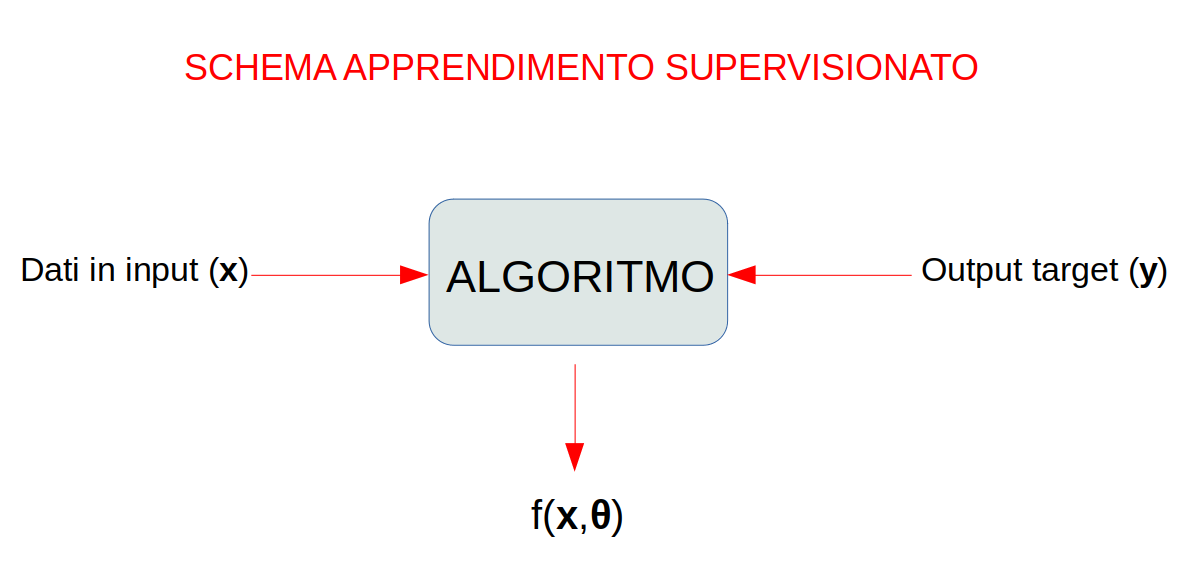
\includegraphics[width=0.85\textwidth]{figs/App_sup.png}
	\caption{si riporta uno schema intuitivo del funzionamento di un algoritmo di apprendimento supervisionato}
	\label{fig:schema_app_sup}
\end{figure}


Per ogni vettore $\vec{x}$ del \textbf{training data set} è possibile definire una particolare funzione detta $\textit{Loss Function}$ $L(\vec{y},f(\vec{x},\vec{\theta}))$. Questa funzione rappresenta una misura della differenza fra l'output dell'algoritmo e quello atteso.\\ 
A questo punto è possibile fare una media di tale funzione sull'intero set di dati a disposizione, ottenendo la funzione di rischio: \\
\begin{equation}
R(\vec{\theta}) = \frac{1}{N}\sum_{k=1}^{N}L(\vec{y},f(\vec{x},\vec{\theta}))
\end{equation}
dove N è il numero di eventi del training data set. \\
Quindi, mentre la \textbf{Loss Function} rappresenta una misura dell'errore compiuto dall'algoritmo nel fornire l'output per un singolo evento di input, la funzione di rischio è una media di tale errore sull'intero campione di dati di addestramento.\\
Un esempio di funzione di rischio molto diffusa è l'errore quadratico medio:
\begin{equation}
R(\vec{\theta}) = \frac{1}{N}\sum_{k=1}^{N}(\vec{y}_k - f(\vec{x}_k , \vec{\theta}))^2
\end{equation}
Quando si addestra un modello si vuole inoltre evitare il così detto $\textit{overfitting}$, che consiste in un eccessivo adattamento del modello ai dati di training e che di conseguenza porta al non raggiungimento di una sufficiente generalità; in tal caso infatti l'algoritmo costruisce una funzione $f(\vec{x},\vec{\theta})$, che ha una forte potenza nella classificazione del campione di addestramento, ma non ha la stessa potenza di classificazione su altri campioni statistici. \\
Un modo per verificare un eventuale overfitting è quello di verificare se il modello è nettamente migliore per il data set di allenamento rispetto al data set di test. \\
Per arginare questo problema è possibile modificare la funzione di rischio, aggiungendo una funzione $Q(\vec{\theta})$; in questo modo si ottiene la funzione di costo:
\begin{equation}
C(\vec{\theta}) = R(\vec{\theta}) + \lambda Q(\vec{\theta})
\end{equation}
con $\lambda$ parametro che esprime la rigidità del vincolo.\\
A questo punto l'obiettivo è quello di minimizzare la funzione di costo ed uno dei metodi più comuni per tale scopo è il metodo di discesa del gradiente.\\
Discesa del gradiente è una tecnica di ottimizzazione utilizzata per minimizzare l'errore che si introduce stimando la $\hat{\vec{y}} = f(\vec{x},\vec{\theta})$ rispetto alla funzione "vera" $\vec{y} = f(\vec{x})$. Un processo di questo tipo è caratterizzato, per quanto detto precedentemente, da una \textbf{Loss Function} $L(\vec{y},f(\vec{x},\vec{\theta}))$ ed un vettore $\vec{\theta}$, le cui componenti sono i parametri che devono essere ottimizzati nel processo di addestramento al fine di ridurre il più possibile l'errore che viene commesso dall'algoritmo nello stimare l'output, rispetto all'output target.\\
Esistono tre varianti del metodo di discesa del gradiente:

\begin{itemize}
	\item $\textit{Batch Gradient Descent}$. \\
	 L'aggiornamento del vettore dei parametri $\vec{\theta}$ avviene una volta sola durante il processo di addestramento e, nello specifico, solo dopo che l'algoritmo ha processato tutto il campione di addestramento degli eventi di input.  Per fare ciò si calcola il vettore $\vec{G}$ come la media su tutto il \textbf{training data set} del gradiente (nello spazio dei parametri) della \textbf{Loss Function}:
	 	\begin{equation}
	 	\vec{G} = \frac{1}{N} \sum_{k=1}^{N} \vec{\nabla}_{\vec{\theta}} L(\vec{y}_k,f(\vec{x}_k,\vec{\theta})) 
	 	\end{equation}
	 e, con tale risultato, viene aggiornato il vettore dei parametri nel seguente modo: 
	 	\begin{equation}
	 	\vec{\theta} - \epsilon\vec{G} \rightarrow \vec{\theta}
	 	\end{equation}
	 Qui $\epsilon$ prende il nome di $\textit{learning rate}$ e regola l'aggiornamento del vettore dei parametri nella direzione opposta a quella del gradiente $\vec{G}$.\\
	 Quindi con questa tecnica si calcola la discesa del gradiente una sola volta, tuttavia si impiega molto tempo per arrivare ad una convergenza ed è quindi poco adatta quando si hanno grandi moli di dati a disposizione. \\
	 
	\item $\textit{Stochastic Gradient Descent}$. \\
	Viene calcolata la discesa del gradiente per ogni pattern fornito all'algoritmo:
	 	\begin{equation}
		\textbf{G}_i =  \boldsymbol{\nabla}_\theta L(\textbf{y}_i,f(\textbf{x}_i,\bm{\theta})) 
		\end{equation}
	e quindi anche l'aggiornamento dei pesi avviene tante volte quanti sono i pattern iniziali:
		\begin{equation}
		\bm{\theta} - \epsilon\textbf{G}_i \rightarrow \bm{\theta}
		\end{equation}
	Questa tecnica è, all'opposto della precedente, utile quando il numero di pattern di input è molto elevato. \\
		
	\item $\textit{Mini Batch Gradient Descent}$. \\
	Si tratta di una via di mezzo fra i due metodi appena presentati perché l'aggiornamento dei pesi avviene più volte dopo che sono stati presentati dei sottogruppi dell'intero data set di addestramento. 
	
\end{itemize}

\color{red}
Chiedere chiarimento su funzione Q($\theta$) \\
termini inglesi \\
spiegazione discesa del gradiente \\
\color{black}

\newpage

%%%%%%%%%%%%%%%%%%%%%%%%%%%%%%%%%%%%%%%%%%%%%%%%%%%%%%%%%%%%%%%

\subsection{Apprendimento non supervisionato}
\label{app_non_sup}

Gli algoritmi di apprendimento supervisionato risultano essere molto utili nel caso in cui si abbiano a disposizione sia i vettori di input che i corrispettivi output target, perché si riesce ad ottenere un'approssimazione della relazione esistente input-output; nel caso della fisica delle alte energie questo significa conoscere le proprietà degli eventi di segnale che si vogliono individuare.\\
Tuttavia nel caso di ricerche ad ampio spettro, che non dipendano fortemente da un modello, e che quindi non hanno una descrizione precisa degli eventi di interesse, non e' possibile avere a priori un campione di segnali con il relativo output di riferimento. \\
In questo caso si può ricorrere all'uso di tecniche di apprendimento non supervisionato, dove l'obiettivo è quello di trovare eventuali partizioni degli input (Clustering), cioè vengono ricercati all'interno degli input quelli che sono diversi dalle aspettative perché hanno proprietà non affini a tutti gli alti eventi del campione. \\
Si consideri la figura \ref{Unsup} dove sono riportate tre diverse configurazioni possibili nel caso di input bidimensionali: nel caso a) è possibile la separazione in due sotto-gruppi e nel caso b) in un unico sotto-gruppo, mentre nel caso c) sembrerebbe non si possano stabilire graficamente eventuali separazioni.

\begin{figure}[h!]
	\centering
	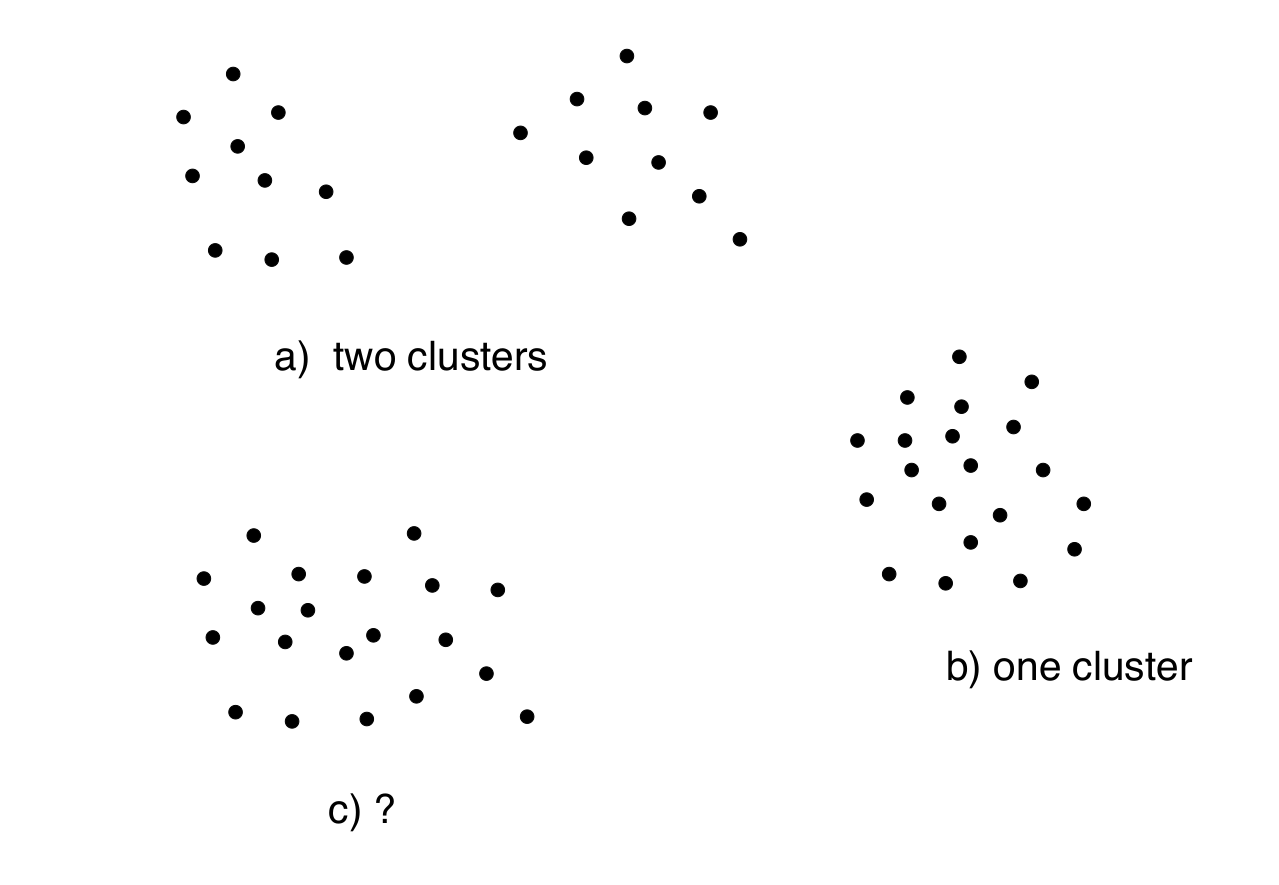
\includegraphics[width=0.85\textwidth]{figs/Unsup_learning.png}
	\caption{vettori di input in uno spazio bidimensionale in tre situazioni differenti. L'immagine è presa da \cite{IntroML}}
	\label{Unsup}
\end{figure}

Quindi un algoritmo di clustering si occupa della suddivisione del set di input $\Sigma$ in un numero N di sottogruppi $\Sigma_1$,...,$\Sigma_n$, detti appunto cluster; si noti che lo stesso numero N non viene stabilito a priori e fornito all'algoritmo, ma viene anch'esso ricavato a partire dai dati. Una volta fatto sarà possibile implementare un classificatore per collegare nuovi vettori di input con i cluster precedentemente individuati.\\
Inoltre, aumentando il livello di complessità, è possibile trovare eventuali gerarchie di partizionamento, ovvero cluster di cluster.\\
Un esempio di clustering è quello basato sulla distanza euclidea. \\
E' di fondamentale importanza osservare che nei metodi che si basano sul concetto di distanza è importante ri-scalare i valori delle componenti degli eventi (in linea di principio si possono avere componenti diverse con ordini di grandezza di molto differenti) in modo da evitare che alcune componenti pesino più di altre. \\
Gli algoritmi di apprendimento non supervisionato sfruttano una misura di similarità per separare gli eventi di input nei vari cluster. Una possibilità è quella di utilizzare la semplice distanza euclidea per poter separare lo spazio n-dimensionale degli eventi in delle sotto-aree (i cluster). \\
Per fare ciò viene implementato un metodo iterativo, basato sulla definizione di alcuni punti particolari nello spazio degli eventi, detti $\textit{cluster seekers}$ (letteralmente "cercatori di cluster"). \\
Si definiscono M punti nello spazio n-dimensionale $\vec{C}_{1},...,\vec{C}_{M}$ e l'obiettivo è quello di fare in modo che ogni punto si muova verso il centro di ogni singolo cluster, in modo che ogni cluster abbia al suo centro uno di questi cluster seekers. Inoltre, dato che il numero di cluster non e' conosciuto a priori, il numero M durante la prima iterazione e' arbitrario. \\
Gli eventi del training data set $\Sigma$ vengono presentati all'algoritmo uno alla volta: per ognuno di essi ($\vec{x}_i$) si cerca il cluster seekers più vicino ($\vec{C}_k$) e lo si sposta verso $\vec{x}_i$ nel seguente modo:
\begin{equation}
\vec{C}_k + \alpha_k(\vec{x}_i - \vec{C}_k) \rightarrow \vec{C}_k
\end{equation}
dove $\alpha_k$ è un parametro di apprendimento che determina di quanto $\vec{C}_k$ si muove verso il punto $\vec{x}_i$. \\
Dato che l'algoritmo deve spostare ciascun $\vec{C}_k$ al centro del cluster k-esimo, i suoi spostamenti devono essere di entità, in media, sempre minore. Per evitare che $\vec{C}_k$ abbia spostamenti sempre più ampi al crescere delle iterazioni si definisce una massa $m_k$ e le si assegna un valore pari al numero di volte in cui $\vec{C}_k$ è stato soggetto a spostamenti (quindi anche il valore della massa verrà aggiornato di volta in volta); dopodiché si assegna ad $\alpha_k$ il seguente valore
\begin{equation}
\alpha_k = \frac{1}{1 + m_k}
\end{equation} 
e, dato che ad ogni iterazione che coinvolge $\vec{C}_k$ il valore di $m_k$ aumenta di una unità, il parametro di apprendimento $\alpha_k$ diminuisce di volta in volta. \\
Il risultato di questo aggiustamento è che il cluster seeker si trova sempre nel punto che rappresenta la media dei punti del cluster. \\
Una volta che sono stati presentati tutti gli eventi del campione di addestramento all'algoritmo, i vari cluster seeker andranno a convergere ai "centri di massa" dei cluster e la classificazione (cioè la delimitazione dei cluster nello spazio n-dimensionale) può essere fatta con una partizione dello spazio di Voronoi, ossia un generico punto (evento) $\vec{x}_i$ viene inserito nel cluster k-esimo se la distanza di tale punto dal cluster seeker $\vec{C}_k$ è minore rispetto alla sua distanza da tutti gli altri cluster seeker. \\
Un esempio didattico del risultato di questa partizione è riportato in figura ~\ref{Voronoi}.

\newpage

\begin{figure}[h!]
	\centering
	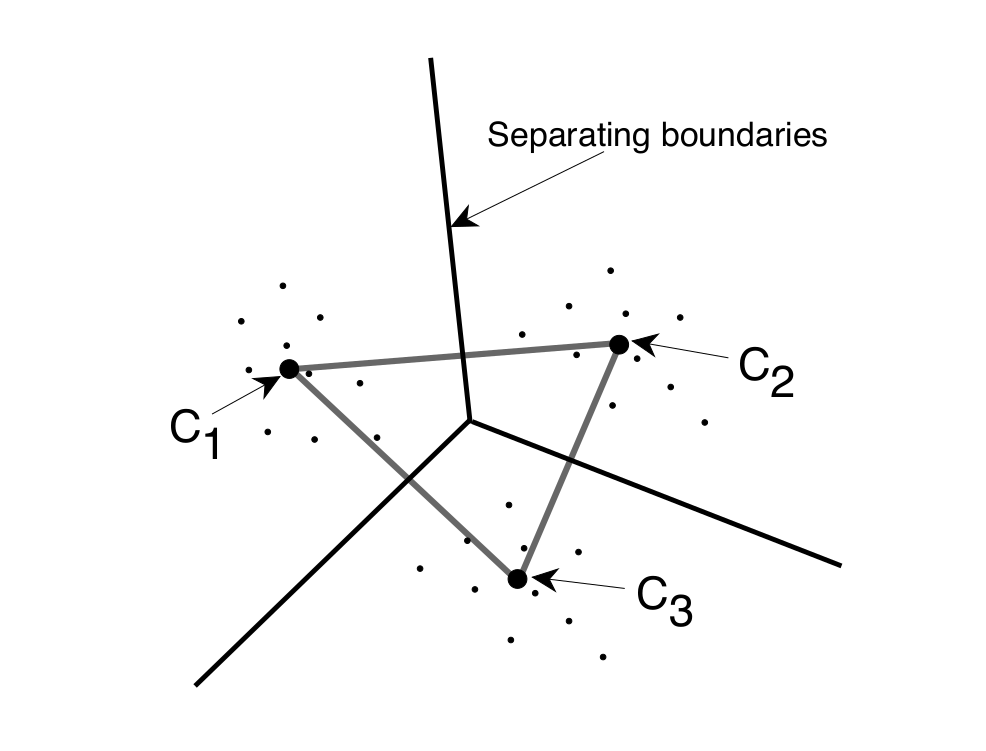
\includegraphics[width=0.70\textwidth]{figs/Voronoi.png}
	\caption{Si riporta un esempio di partizione dello spazio (bi-dimensionale) di Voronoi in tre sotto regioni, dove i punti $C_1$, $C_2$ e $C_3$ sono i cluster seeker. L'immagine è presa da \cite{IntroML}}
	\label{Voronoi}
\end{figure}

Si è accennato qualche riga fa che il numero di cluster seeker è inizialmente scelto in maniera casuale, per poi essere ottimizzato; per il processo di ottimizzazione si utilizza la varianza degli eventi $\vec{x}_i$ per ogni cluster:
\begin{equation}
\sigma^2 = \frac{1}{L}\sum_{i=1}^{L} (\vec{x}_i - \vec{\mu})^2
\end{equation}
dove L è il numero di eventi nel cluster e $\vec{\mu}$ ne è la media:
\begin{equation}
\vec{\mu} = \frac{1}{L}\sum_{i=1}^{L} \vec{x}_i
\end{equation}
A questo punto, se la distanza $d_{ij}$ fra due cluster seeker $\vec{C}_i$ e $\vec{C}_j$ è minore di un determinato valore $\epsilon$, allora si sostituiscono i due cluster seeker con uno nuovo posto nel loro centro di massa (tenendo conto delle due masse $m_i$ e $m_j$); dall'altro lato, se vi è un cluster per il quale la varianza $\sigma^2$ è più grande di un valore $\delta$, si aggiunge un nuovo cluster seeker vicino a quello già esistente e si eguagliano entrambe le loro masse a zero.\\
Come osservazione finale bisogna dire che nei metodi che si basano sul concetto di distanza è importante ri-scalare i valori delle componenti dei pattern (in linea di principio si possono avere componenti diverse con ordini di grandezza di molto differenti) in modo da evitare che alcune componenti pesino più di altre. \\ 

\color{red}
Come definisco la misura\\
Riscalare le componenti è importante... che riferimento devo fare alla fisica delle particelle? \\
come scelgo il valore di $\epsilon$ e di $\delta$?
\color{black}


\newpage

%%%%%%%%%%%%%%%%%%%%%%%%%%%%%%%%%%%%%%%%%%%%%%%%%%%%%%%%%%%%%%%

\subsection{Iperparametri e Grid Search}
\label{iperparametri e grid search}

Un modello di apprendimento è caratterizzato da una serie di parametri che vengono modificati in maniera iterativa in modo da minimizzare la \textbf{Loss function} e tale processo avviene attraverso un continuo confronto con il \textbf{training data set}.\\ 
Gli iperparametri sono invece una serie di parametri che caratterizzano il modello implementato che non sono modificati nel processo di addestramento ma vengono prestabiliti dall'utente. Gli iperparametri rappresentano delle caratteristiche dell'algoritmo, che possono essere modificate prima di avviare il processo di addestramento, come ad esempio il numero di neuroni in una rete neurale (\ref{reti neurali}), oppure il numero di epoche, cioè il numero di volte in cui viene ripresentato all'algoritmo l'intero campione di dati di addestramento.\\
E' molto probabile che ci siano configurazioni di iperparametri migliori di altre, cioè per le quali l'addestramento dell'algoritmo produce esiti migliori; di conseguenza anche gli iperparametri devono essere sottoposti ad un processo di ottimizzazione. \\
Uno dei metodi utilizzati per tale scopo è il \textit{Grid Search}, che è piuttosto semplice da implementare nella pratica. Fa parte dei così detti \textit{Brute-Force Search}, cioè di quei metodi che si basano sulla sistematica verifica di tutte le possibili soluzioni ad un problema per poi considerare la migliore. Per esempio si consideri il problema di dover cercare i divisori di un numero n: un approccio "Brute-Force" prevedrebbe di considerare tutti i numeri minori di n e verificare quelli per i quali la divisione non dà resto. Questo esempio permette anche di mettere in evidenza il limite principale di tale tipologia di approccio: il numero di possibilità da esplorare può aumentare molto velocemente, soprattutto se si considera un processo multivariato. \\
Per il Grid Search si consideri un modello caratterizzato da un numero k di iperparametri, quindi e' possibile creare un vettore le cui componenti siano gli iperparametri stessi:
\begin{equation}
\vec{\mu} = (\mu_1,...,\mu_k)
\end{equation}
Tale vettore appartiene ad uno spazio k-dimensionale, sul quale può essere costruita una griglia i cui nodi corrispondono a particolari combinazioni degli iperparametri. \\
A questo punto si può avviare l'apprendimento del modello per ogni particolare configurazione degli iperparametri ed ottenere un valore per la \textbf{Loss function}, e quindi la miglior configurazione sarà quella che minimizza tale funzione. \\
In Figura~\ref{fig:Grid Search} nella pagina seguente è riportato per chiarezza un esempio visivo dell'esito di un processo di ottimizzazione degli iperparametri attraverso il metodo Grid Search.

\begin{figure}[h!]
	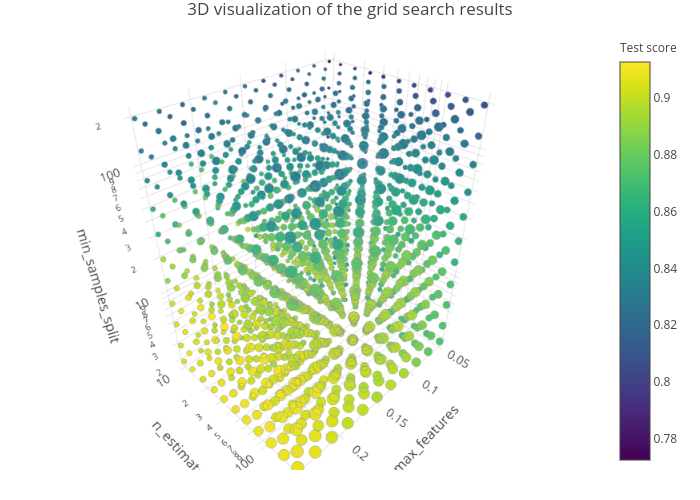
\includegraphics[width=\linewidth]{figs/Grid_immagine.png}
	\caption{la figura illustra visivamente l'esito di un processo di ottimizzazione degli iperparametri attraverso il metodo Grid Search \cite{knuthwebsite}}
	\label{fig:Grid Search}
\end{figure}
\newpage 

Come accennato precedentemente, man mano che aumenta la complessità del modello è molto probabile che aumenti il numero degli iperparametri e quindi la dimensionalità dello spazio introdotto precedentemente; ciò implica l'aumento considerevole del numero di configurazioni degli iperparametri da esplorare attraverso il Grid Search e quindi il tempo necessario per concludere l'ottimizzazione.\\
E' possibile ovviare parzialmente a questo problema attraverso il Random Grid Search (RGS), dove non sono considerati tutti i nodi della griglia, ma solo una loro parte selezionata in maniera casuale secondo una particolare distribuzione, scelta in modo arbitrario al momento dell'implementazione del RGS. \\
Un ulteriore accorgimento può  essere quello di bloccare l'ottimizzazione di alcune configurazioni che sembrano meno promettenti, ad esempio quando superano un certo valore della \textbf{Loss function}, evitando che il processo di apprendimento venga completato su tutti i nodi. Per far ciò, è possibile implementare degli $\textit{scheduler}$ che tengano conto dell'andamento dei diversi training relativi alle diverse configurazioni. Un approccio diverso è quello di esplorare nuove varianti a partire dalle configurazioni iniziali. In quest'ultimo caso non è nemmeno necessario definire in modo rigido lo spazio degli iperparamentri da esplorare dato che le nuove configurazioni vengono ricercate a partire dall'andamento delle precedenti ($\textit{popultion based training}$).

\newpage

%%%%%%%%%%%%%%%%%%%%%%%%%%%%%%%%%%%%%%%%%%%%%%%%%%%%%%%%%%%%%%%%

\subsection{Reti Neurali}
\label{reti neurali}
Le reti neurali sono probabilmente il metodo di apprendimento supervisionato più conosciuto ed utilizzato nel campo dell'analisi dati. \\
La struttura di una rete neurale prevede la presenza di unità fondamentali, dette neuroni, che sono organizzate in strati e legate fra di loro mediante delle connessioni (sinapsi), ciascuna delle quali è caratterizzata da un peso. Sono proprio questi pesi a giocare un ruolo fondamentale nel processo di apprendimento della rete perché sono loro i parametri soggetti a modifica.\\
Il nome rete neurale (artificiale) deriva dal fatto che la loro struttura è inspirata dalle corrispondenti strutture biologiche. \\
In una rete neurale è sempre presente uno strato di input ed uno di output, mentre il numero di livelli nascosti può variare a seconda della complessità della rete; In figura \ref{fig:schemaNN} è riportato un esempio di rete neurale con un singolo strato interno nascosto.
\begin{figure}[h!]
	\centering
	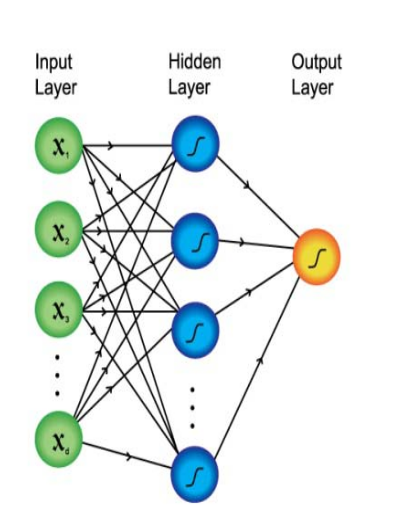
\includegraphics[width=0.50\textwidth]{figs/schemaNN.png}
	\caption{si riporta un esempio grafico di rete neurale formata da un unico strato nascosto. L'immagine è presa da \cite{Metodi_multivariati}.}
	\label{fig:schemaNN}
\end{figure}
\\
Si può passare ora a presentare il modello del singolo neurone per capire com'è strutturato e quale compito svolge.
Gli elementi che caratterizzano il singolo neurone sono:
\begin{enumerate}
	\item Una serie di connessioni in ingresso (ciascuna caratterizzata da un proprio peso);
	\item Un sommatore che ha il compito di svolgere la somma pesata degli input, utilizzando i pesi caratteristici delle connessioni;
	\item Un output e la relativa funzione di attivazione, che viene usata per limitarne l'ampiezza (tipicamente ad intervalli [0,1] o [-1,1]);
	\item Un valore di soglia che viene usato per aumentare o diminuire il valore ottenuto dalla somma pesata.
\end{enumerate}
Si riporta in figura \ref{schema_neurone} lo schema grafico di un singolo neurone (k), dove $\vec{x} = (x_1 ,..., x_m)$ è il vettore degli input input, $\vec{w}_k = (w_{k1} ,..., w_{km})$ è il vettore dei pesi, $\phi$(x) è la funzione di attivazione, $b_k$ è il valore di soglia e $y_k$ è l'output.
\begin{figure}[h!]
	\centering
	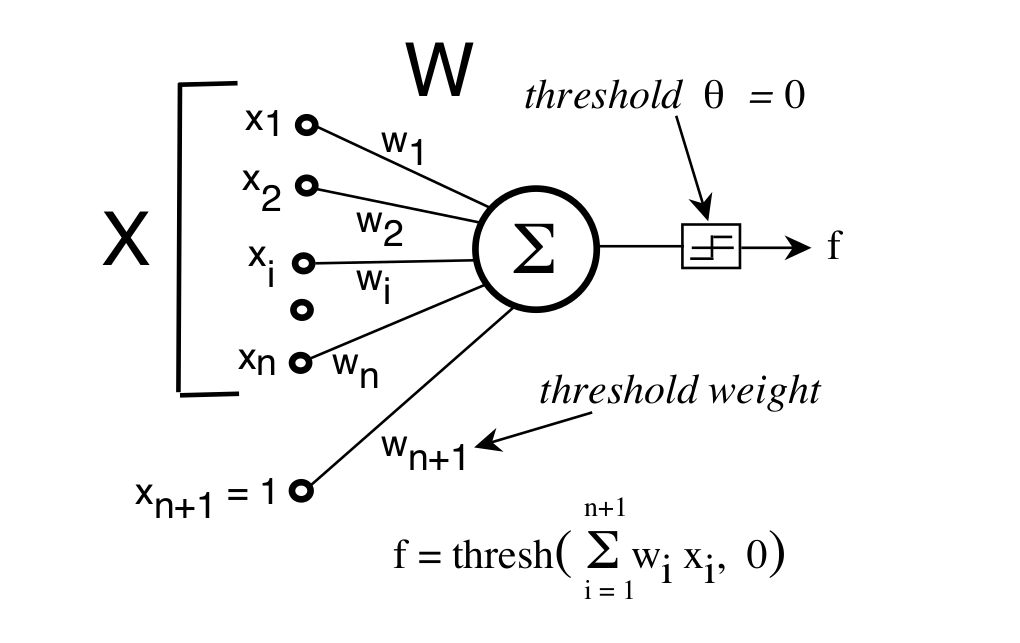
\includegraphics[width=0.70\textwidth]{figs/schema_neurone.png}
	\caption{Illustrazione della struttura di un neurone \cite{Intro_retiN}.}
	\label{schema_neurone}	
\end{figure} \\
Quindi il neurone opera la seguente somma pesata:
\begin{equation}
s_k = \vec{x}\bullet\vec{w}_\textbf{k} = \sum_{i=1}^{m}x_iw_{ki}
\label{sk}
\end{equation}
e si ottiene l'output attraverso la funzione di attivazione: 
\begin{equation}
y_k = \phi(s_k + b_k)
\end{equation}
Risulta utile spendere qualche parola in più sul tipo di funzione di attivazione più utilizzata, ovvero la funzione sigmoide:
\begin{equation}
sig(x) = \frac{1}{1 + e^{-{\alpha}x}}
\end{equation} 
dove $\alpha$ è un parametro che permette di regolare la pendenza della curva, come si evince dalla figura ~\ref{sigmoide}
\begin{figure}[h!]
	\centering
	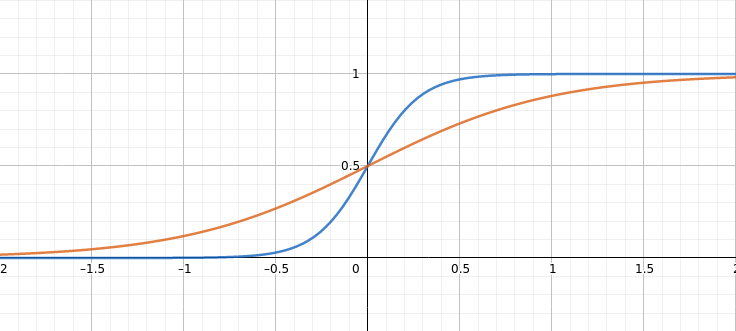
\includegraphics[width=0.75\textwidth]{figs/sigmoide.png}
	\caption{Si riportano due sigmoidi, dove per quella in rosso si ha $\alpha$=2 e per quella in blu $\alpha$=7.}
	\label{sigmoide}
\end{figure}
\newpage
Un singolo neurone è l'ingrediente fondamentale di una rete neurale e nella gran parte dei casi non è in grado di ottenere da solo nessuna classificazione degli input. Tuttavia esiste una caso particolare nel quale un singolo neurone può portare a termine un compito di classificazione; affinché ciò sia possibile è necessario che i vettori evento siano riconducibili a due sole categorie e che il loro spazio possa essere separato (in relazione alle due categorie) da un singolo iper-piano. In questo caso esiste un teorema di convergenza che garantisce la convergenza dei pesi nel processo di addestramento.

A questo punto è possibile passare ad un livello di complessità superiore, osservando in che modo possono essere organizzati i neuroni per formare la rete neurale; si distinguono due tipologie di reti:
\begin{enumerate}
	\item Reti feedforward con uno o più strati: in questo caso il segnale si propaga dai nodi di input verso quelli di output, senza connessioni fra i neuroni di uno stesso strato;
	\item Reti feedback: sono reti cicliche dove il segnale si propaga anche fra i neuroni di uno stesso strato.
\end{enumerate}
L'apprendimento di un singolo neurone dipende dalla struttura della rete e dal tipo di input ed output fornito alla rete. Nel caso in cui l'output target sia noto si può utilizzare il metodo dell'apprendimento con correzione di errore. \\
Si consideri un singolo neurone che ha in ingresso una serie di input $(x_1,...,x_n)$ e quindi produce un valore di output $y$ attraverso la somma pesata già introdotta precedentemente; tale valore può quindi essere confrontata con il risultato atteso $R$, ottenendo così un errore $err = R - y$; si può quindi definire la funzione di costo
\begin{equation}
E = \frac{1}{2}err^2
\end{equation}
sulla quale si applicherà il metodo di discesa del gradiente già discusso nel paragrafo~\ref{discesa del gradiente} per ottimizzare i parametri.\\
Una rete neurale può svolgere diverse funzioni, tuttavia quella principale che viene utilizzata in questa tesi prende il nome di riconoscimento. Il riconoscimento consiste nell'associazione da parte della rete di un vettore evento ad una delle varie categorie possibili. Tale obiettivo può essere ottenuto a seguito di una fase di addestramento dove vengono forniti alla rete sia i vettori in input che le categorie alle quali questi appartengono (si tratta chiaramente di un processo di apprendimento supervisionato). Si ipotizzi di avere a disposizione dei vettori evento con un numero n di componenti (i dati) che rappresentano dei punti in uno spazio n-dimensionale; questo spazio potrà essere allora diviso in delle regioni che corrispondono alle varie categorie ed i confini di queste regioni si ottengono a seguito del processo di addestramento. \\
Durante l'addestramento ogni singolo neurone deve aggiornare i suoi pesi in modo che l'output della rete sia simile a quello atteso. \\
Uno dei metodi migliori per addestrare la rete neurale è l'algoritmo di back-propagation. \\
Per l'implementazione di questo algoritmo si introduce un segnale di input che deve propagarsi verso lo strato di output e, allo stesso tempo, si fa propagare un segnale di errore dallo strato di output verso quello di input.\\
Nel caso della back-propagation bisogna fare una distinzione tra l'addestramento dei neuroni nello strato di output e negli strati nascosti:
\begin{enumerate}
	\item Neurone nello strato di output.\\
	Un neurone di output k, quando gli verrà fornito l'elemento j del \textbf{training data set}, avrà un errore:
	\begin{equation}
	err_k^{(j)} = R_k^{(j)} - y_k^{(j)}
	\end{equation}
	dove con la lettera y si intende il valore ottenuto in output dal neurone e con R il valore atteso. \\
	L'errore totale dello strato di output per il vettore evento j-esimo viene definito nel seguente modo:
	\begin{equation}
	E^{(j)} = \frac{1}{2} \sum_{k=1}^{n} (err_k^{(j)})^2
	\end{equation}
	dove n è il numero di neuroni nello strato di output. \\
	Se poi N è il numero totale di elementi del training data set, allora la funzione di costo può essere definita nel seguente modo:
	\begin{equation}
	E_{tot} = \frac{1}{N}\sum_{j=1}^{N} E^{(j)}
	\end{equation}
	e l'obiettivo è quello di minimizzare tale funzione di costo. Per fare ciò si procede variando i pesi a seguito della presentazione di ogni singolo vettore evento.
	Si utilizza il metodo di discesa del gradiente, procedendo nel seguente modo: il gradiente è dato da
	\begin{equation}
	\frac{\partial E^{(j)} }{\partial w_{ki}^{(j)}}
	\end{equation}
	e gli aggiornamenti del peso vengono applicati nel verso opposto del gradiente, ovvero
	\begin{equation}
	\Delta w_{ki}^{(j)} = -\mu \frac{\partial E^{(j)} }{\partial w_{ki}^{(j)}}
	\end{equation}
	con $\mu$ fattore di apprendimento, definito precedentemente come $\textit{learning rate}$.
	Manca a questo punto il calcolo esplicito del gradiente, che può essere eseguito con la regola della catena 
	\begin{equation}
	\frac{\partial E^{(j)} }{\partial w_{ki}^{(j)}} = \frac{\partial E^{(j)}}{\partial err_k^{(j)}}
	\frac{\partial err_k^{(j)}}{\partial y_k^{(j)}}
	\frac{\partial y_k^{(j)}}{\partial S_k^{(j)}}
	\frac{\partial S_k^{(j)}}{\partial w_{ki}^{(j)}}
	\end{equation}
	dove $S_k^{(j)} = s_k^{(j)} + b_k^{(j)} $ (si faccia riferimento all'equazione \eqref{sk}). \\
	Una volta calcolate le quattro derivate si ottiene:
	\begin{equation}
	\frac{\partial E^{(j)} }{\partial w_{ki}^{(j)}} =
	-err_k^{(j)}\phi'(S_k^{(j)})y_i^{(j)}
	\end{equation}
	e quindi:
	\begin{equation}
	\Delta w_{ki}^{(j)} = err_k^{(j)}\phi'(S_k^{(j)})y_i^{(j)} \mu
	\end{equation}
	
	\item Neurone in uno strato nascosto \\
	In questo caso l'output del neurone non ha un diretto valore con il quale può essere confrontato, quindi il segnale di errore deve essere determinato a partire dai segnali di errore di tutti i neuroni dello strato successivo, da cui il nome di back-propagation proprio perché il segnale di errore prosegue all'indietro dall'output verso l'input.
\end{enumerate}
Come ultima considerazione sulle reti neurali bisogna sottolineare che il fattore di apprendimento deve essere scelto in maniera accurata, infatti se fosse troppo piccolo si avrebbe una convergenza estremamente lenta e, viceversa, un valore troppo grande porterebbe ad una instabilità con comportamento oscillatorio. Per gestire meglio questo aspetto, nella pratica viene definito un learning rate variabile. Generalmente si fa in modo che questo fattore parta da un certo valore per decrescere mano mano che si ci avvicina ad una soluzione ottimale. In prima istanza infatti è utile avere un valore abbastanza grande da poter seguire in modo efficace la discesa del gradiente, rendendo più rapida la ricerca della soluzione ottimale. Successivamente, però, risulta utile diminuire questo stesso parametro per evitare oscillazioni attorno al punto di minimo.

\color{red}
ultimo commento reti neurali $\rightarrow$ il fattore di apprendimento l'ho definito e si vede dove appare nella backpropagation \\
\color{black}

\newpage

%%%%%%%%%%%%%%%%%%%%%%%%%%%%%%%%%%%%%%%%%%%%%%%%%%%%%%%%%%%%%%%%

\subsection{Alberi Decisionali}
\label{alberi decisionali}
Gli alberi decisionali sono, al pari delle reti neurali, un metodo ML di apprendimento supervisionato.\\
Gli alberi decisionali rappresentano un mezzo estremamente interessante per le operazioni di classificazione (sia per output continui che discreti) ed operano attraverso una serie di test sugli attributi degli eventi di input. \\ 
Come primo passo è utile discutere come è strutturato un albero decisionale, introducendo alcune notazioni (come ausilio alla trattazione si riporta in figura \ref{schemaDT} un esempio di albero decisionale molto semplice). \\

\begin{figure} [h!]
	\centering
	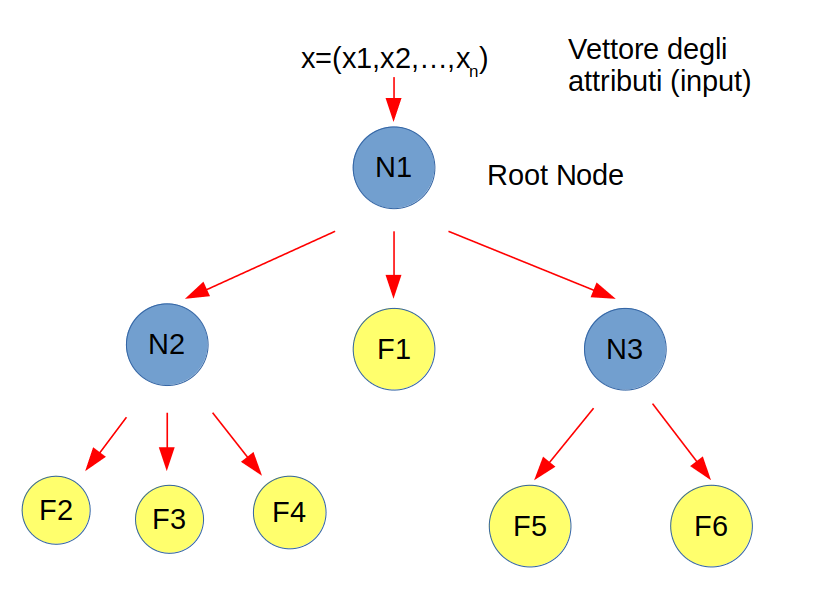
\includegraphics[width=0.70\textwidth]{figs/schemaDT.png}
	\caption{esempio di come è strutturato un albero decisionale}
	\label{schemaDT}
\end{figure} 

Gli elementi che caratterizzano un albero decisionale sono:
\begin{itemize}
	\item Nodo. \\
	I nodi sono riportati in figura \ref{schemaDT} come dei cerchi colorati in azzurro e contrassegnati dalla lettera N. Ogni nodo si occupa di eseguire un test su di un singolo attributo (il nodo iniziale dove avviene il primo test e quindi la prima differenziazione degli input è detto "root node");
	\item Ramo. \\
	I rami (detti anche archi) determinano le regole di "splitting", ovvero le regole attraverso le quali vengono separati gli esempi nelle rispettive categorie a seconda dei loro attributi; tali rami determinano quindi i percorsi all'interno degli alberi decisionali e la classificazione finale;
	\item Foglie. \\
	Le foglie sono una classe particolare di nodi, ovvero i nodi finali che, in quanto tali, non generano nuove diramazioni ma rappresentano il risultato finale del processo di classificazione.
\end{itemize}

Nella costruzione degli alberi decisionali bisogna distinguere due fasi successive:
\begin{itemize}
	\item "Building", ovvero costruzione.\\
	In questo prima fase l'obiettivo è quello di far crescere l'albero in dimensione, quindi in termini di rami e nodi per avere un numero adeguato di regole di splitting così da ottenere una classificazione in classi omogenee nella fase finale. In questa prima fase si ottiene un albero particolarmente folto e quindi probabilmente soggetto all'overfitting (come primo argine a ciò è possibile introdurre un criterio d'arresto capace di fermare la crescita dell'albero al realizzarsi di particolari condizioni);
	\item "Pruning", ovvero potatura.\\
	Questa fase è quella che permette di ridurre l'overfitting perché vengono eliminati i rami che non contribuiscono in maniera significativa al processo di classificazione.
	
\end{itemize} 

Poiché ciascun nodo agisce su una singola variabile dei vettori di input, è possibile ottenere un gran numero di alberi differenti. Per questo motivo è necessario trovare un modo per ottimizzare la geometria dei nodi all'interno dell'albero: per farlo viene scelto per primo l'attributo attraverso il quale si ha una maggiore discriminazione dei dati in input. Per fare ciò si possono percorrere due strade distinte, utilizzando:
\begin{itemize}
	\item Coefficiente di impurità di Gini, ovvero un indicatore della frequenza con cui un elemento casuale, appartenente al data set, sia identificato in modo non corretto.
	\item Guadagno informativo, ovvero un indicatore, preso in prestito dalla teoria dell'informazione e basato sul concetto di entropia, di quanto la scelta di uno specifico attributo consenta di ridurre l’entropia informativa dell'insieme (semplificando, la variabilità dei valori dell'attributo presenti all'interno di un nodo foglia). 
\end{itemize}  

E' chiaro che entrambi questi indici vengono utilizzati con la stessa finalità, tuttavia ogni algoritmo ha una differente logica di costruzione e quindi adotterà uno solo dei due indici, con la possibilità di ottenere risultati differenti. \\
Una volta costruito l'albero decisionale, i metodi per il \textbf{pruning} sono sostanzialmente due: da un lato si può seguire un approccio "top-down", partendo dalla radice e suddividendo l'intera struttura in sotto alberi e dall'altro un approccio "bottom-up", partendo dalle foglie ed analizzando l'impatto di ogni singola potatura. E' altresì possibile introdurre nella fase di costruzione stessa un criterio di $\textbf{early-stopping}$ o $\textbf{pre-pruning}$ richiedendo un valore minimo di miglioramento dell'algoritmo fra un'iterazione e l'altra: ad ogni passaggio di separazione dell'albero decisionale viene fatto un controllo sulla \textbf{Loss function} e, se tale errore non diminuisce significativamente tra un passaggio e l'altro, si interrompe il processo di costruzione dell'albero. Il problema dell'\textbf{early stopping} è che non tiene conto dell'impatto della selezione sui nodi successivi; per questa ragione in genere si utilizzano entrambi i metodi di $\textbf{pruning}$ e di $\textbf{early stopping}$ parallelamente, per poi confrontare i risultati. \\

Gli alberi decisionali hanno vari pregi, fra i quali quello di essere caratterizzati da una particolare semplicità nell'interpretazione e nella visualizzazione, ed essere insensibili ad eventuali componenti degli eventi irrilevanti nella classificazione; inoltre sono caratterizzati da una tolleranza ad eventuali attributi mancanti per alcuni input nel \textbf{training data set} o nel \textbf{test data set} e da una invarianza per trasformazioni monotone effettuate sulle variabili degli input, che rende la fase di pre-processamento dei dati non necessaria. Dall'altro lato ci sono una serie di limiti, come l'instabilità rispetto al variare del \textbf{training data set}, cioè data set di allenamento di poco differenti fra loro producono risultati molto diversi, oppure il frequente problema dell'\textbf{overfitting}. \\
E' possibile anche combinare più alberi decisionali insieme per ottenere migliori prestazioni predittive. Una delle tecniche per tale combinazione è il $\textit{Bagging}$, dove vengono generati in maniera casuale dei sottogruppi del training data set ed ognuno di questi viene utilizzato per l'addestramento di un albero decisionale. Il risultato sarà una collezione di alberi decisionali e, come decisione finale, si utilizzerà la media delle decisioni dei singoli alberi. \\
Esiste un'estensione di questo metodo conosciuta con il nome di $\textit{Random Forest}$; in questo caso viene aggiunto un passaggio ulteriore al processo appena illustrato perché viene scelto casualmente anche un sottogruppo delle componenti dei vettori di evento, ottenendo così un metodo capace di agire anche su data set ad alta dimensionalità e che permette di ridurre sensibilmente il problema dell'\textbf{overfitting}.

\color{red}
feature o attributo io li intendo come le componenti dei vettori evento in input... cosa c'entrano le distribuzioni ?
\color{black}

\newpage

%%%%%%%%%%%%%%%%%%%%%%%%%%%%%%%%%%%%%%%%%%%%%%%%%%%%%%%%%%%%%%%%

\subsection{Curse of dimensionality e riduzione della dimensionalità}
\label{curse_dim}

I metodi di apprendimento supervisionato, come descritto, necessitano anche di output target per essere addestrati. Nel caso questi non fossero disponibili l'unica soluzione è utilizzare un metodo non supervisionato di ML. Un moderno esempio e' il Variational Autoencoder, di cui nel capitolo \ref{fisica_BSM_VAEs} verrà mostrata un'applicazione nel campo della fisica delle alte energie. \\
Quando si parla di eventi di input ci si riferisce a dei vettori, le cui componenti sono i dati veri e propri; questi vettori, in quanto tali, possono essere pensati all'interno di un opportuno spazio n-dimensionale (con n=numero di componenti del vettore).\\
Spesso, nel campo della fisica delle particelle, il numero di variabili che descrivono ciascun evento e' molto grande e  questo fa si che lo spazio di riferimento sia ad altissima dimensionalità. Come visto, in molti metodi l'aumento della dimensionalità crea delle problematiche riguardo la complessità dell'algoritmo e del tempo di computazione necessario per ottenere dei metodi ottimizzati. Questa problematica prende il nome di \textit{Curse of Dimensionality}. \\
All'aumentare della dimensionalità la densità degli eventi nello spazio diminuisce, e questo fa si che il numero di dati necessari per poter avere dei risultati statisticamente significativi aumenta enormemente. Tutto ciò ha un grande impatto soprattutto quando si vuole fare una classificazione di eventi molto rari.\\
Per ovviare a questo problema si possono utilizzare tecniche attraverso le quali viene ridotto il numero di variabili che caratterizzano gli eventi.; l'obiettivo di base è quello di proiettare gli elementi dello spazio n-dimensionale (i vettori di input) su di uno spazio a dimensione inferiore, limitando il più possibile la perdita di informazione.\\
Degli input con più bassa dimensionalità permettono di avere anche meno parametri (gradi di libertà) e quindi una struttura più semplice del modello. Inoltre sistemi meno complessi sono meno soggetti all'\textbf{overfitting}, oltre a garantire una migliore efficacia statistica. \\
Il processo di riduzione della dimensionalità è una metodologia di preparazione dei dati, per poi essere presentati all'algoritmo di apprendimento, che si troverà di fronte delle informazioni più compatte e quindi più facilmente processabili. Inoltre se tale processo viene svolto sul \textbf{training data set}, allora deve essere attuato anche sul \textbf{test data set}, per garantire un processo di verifica valido.

\newpage

Il processo di riduzione della dimensionalità può essere portato avanti attraverso due metodologie differenti:
\begin{itemize}
	\item Selezione, dove solo alcune componenti dei vettori di input vengono conservate;
	\item Estrazione, dove viene creato un numero ridotto di nuove componenti a partire da quelle originali.
\end{itemize}
A prescindere da questa distinzione, bisogna sottolineare che tutti i processi di riduzione della dimensionalità hanno una struttura comune, ovvero sono caratterizzati da una fase di $\textit{encoding}$ (che rappresenta il vero e proprio processo di riduzione della dimensionalità) e da una fase di $\textit{decoding}$, nella quale si verifica quanta informazione è stata persa nel processo. \\ 
Si riporta in figura \ref{encoder-decoder} l'illustrazione grafica del processo $\textit{encoding-decoding}$
\begin{figure}[h!]
	\centering
	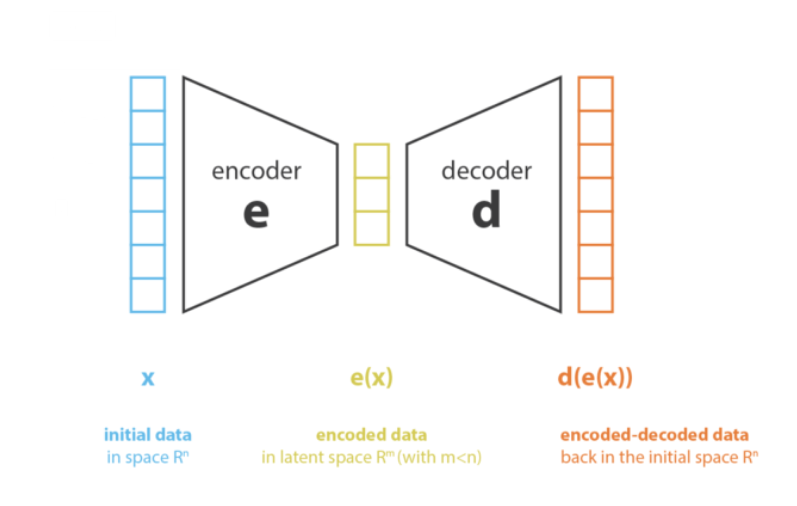
\includegraphics[width=0.90\textwidth]{figs/encoder-decoder.png}
	\caption{Strutture generale di un processo di riduzione della dimensionalità . L'immagine è presa da \cite{Understanding_VAEs}}
	\label{encoder-decoder}
\end{figure}

Il vettore di input $\vec{x}$ (n-dimensionale) viene compresso dall'encoder $\textbf{e}$ in un vettore $\textbf{e}(\vec{x})$ di uno spazio m-dimensionale (con m<n), detto $\textit{spazio latente}$. \\
Il decoder $\textbf{d}$ svolge la funzione opposta, ovvero decomprime il vettore $\textbf{e}(\vec{x})$ in $\textbf{d}(\textbf{e}(\vec{x}))$ per tornare allo spazio originario n-dimensionale. \\
Nel caso in cui $\vec{x} = \textbf{d}(\textbf{e}(\vec{x}))$ (caso ideale) si dice che il processo è un $\textit{lossless encoding}$, ovvero non c'è stata perdita di informazioni nella riduzione della dimensionalità; viceversa, se $\vec{x} \not= \textbf{d}(\textbf{e}(\vec{x}))$, si parla di un $\textit{lossy encoding}$, cioè un processo nel quale parte dell'informazione viene persa e non può essere recuperata con la fase di decodifica. \\
\newpage
Come conseguenza di ciò che è stato appena illustrato, l'obiettivo di un processo di riduzione della dimensionalità è quello di trovare la coppia encoder-decoder (e,d) fra una famiglia di encoder E e di decoder D, che minimizzi l'informazione persa:
\begin{equation}
(e,d) = \min_{E \times D} \epsilon (\vec{x},\textbf{d}(\textbf{e}(\vec{x})))
\end{equation}
dove $\epsilon (\vec{x},\textbf{d}(\textbf{e}(\vec{x})))$ è la grandezza attraverso la quale viene  quantificata la quantità di informazione persa nel processo di riduzione. \\
I metodi di selezione ("$\textit{Feature Selection Methods}$ (FSM)") sono metodi attraverso i quali vengono selezionate le componenti dei vettori di input da tenere e quelle da eliminare perché irrilevanti per le analisi successive. I FSM si includo i $\textit{wrapper methods}$ ed i $\textit{filter methods}$: i primi valutano il modello con varie combinazioni di subset delle variabili originali e selezionano quella per la quale si ha la maggiore accuratezza del modello, mentre i secondi si basano maggiormente sulle caratteristiche intrinseche dei dati (correlazioni, contenuto informativo, etc...). \\
I metodi di estrazione, invece, si basano fortemente sull'algebra lineare; in particolare vengono utilizzati spesso per la riduzione della dimensionalità i metodi di fattorizzazione delle matrici per cogliere la parte più importante dei dati, cioè quella per la quale la perdita di informazione nel processo di ricostruzione è minore. \\
Il più comune di questi metodi prende il nome di $\textit{Principal Component Analysis}$ (PCA). L'idea del PCA è quella di costruire un numero $\textit{n}_\textit{e}$ di nuove variabili indipendenti che siano combinazione lineare delle $\textit{n}$ variabili di partenza; tale costruzione viene fatta in modo tale che la proiezione delle vecchie variabili sul nuovo sottospazio generato da quelle nuove sia il più possibile vicina ai dati iniziali, dove la vicinanza è da intendere in termini della distanza euclidea. In altre parole con il PCA si ricerca il sottospazio dello spazio degli eventi di partenza per il quale l'errore che viene compiuto nell'approssimazione dei dati tramite proiezioni sia il più piccolo possibile. Un esempio grafico è riportato in figura \ref{PCA}.
\begin{figure}[h!]
	\centering
	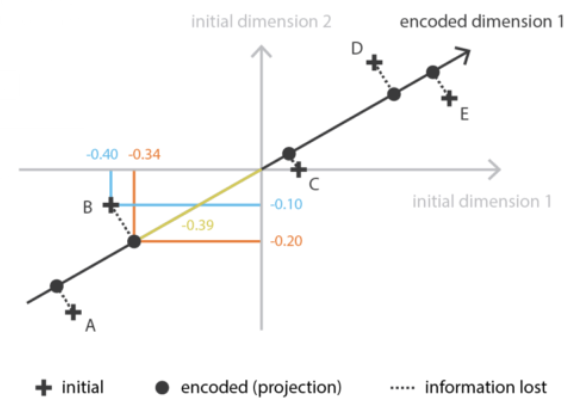
\includegraphics[width=0.70\textwidth]{figs/PCA.png}
	\caption{Illustrazione del processo di PCA nel caso di uno spazio dei pattern iniziali bi-dimensionale \cite{Understanding_VAEs}.}
	\label{PCA}
\end{figure}

\newpage

%%%%%%%%%%%%%%%%%%%%%%%%%%%%%%%%%%%%%%%%%%%%%%%%%%%%%%%%%%%%%%%

\subsection{Autoencoders}
\label{autoencoders}

Gli autoencoders, come ogni altro metodo di riduzione della dimensionalità, sono costituiti da un encoder e da un decoder; tuttavia in questo caso la peculiarità è che sia l'encoder che il decoder sono delle reti neurali, come è possibile vedere in figura ~\ref{autoencoder}. 

\begin{figure}[h!]
	\centering
	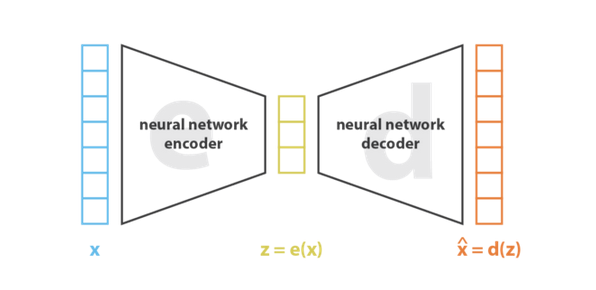
\includegraphics[width=0.70\textwidth]{figs/autoencoder.png}
	\caption{Struttura di un generico autoencoder \cite{Understanding_VAEs}.}
	\label{autoencoder}
\end{figure}

L'obiettivo è anche in questo caso quello di individuare la coppia encoder-decoder che ottimizza il processo di ricostruzione degli input e ciò viene fatto attraverso il seguente processo iterativo: si presentano all'encoder gli eventi di input uno alla volta, subiscono un processo di riduzione della dimensionalità e poi vengono ricostruiti (tornando alla dimensionalità di partenza), viene calcolato l'errore dal confronto fra l'input iniziale e quello ricostruito ed avviene l'aggiornamento dei pesi della rete neurale mediante il meccanismo di backpropagation, già incontrato nella sezione \ref{reti neurali}. \\
Intuitivamente l'autoencoder può essere pensato come un collo di bottiglia, attraverso il quale solo una parte dell'informazione riesce a passare oltre e a formare i vettori dello spazio latente.
Facendo riferimento alla figura \ref{autoencoder} si osserva che, a partire dagli eventi di input $\vec{x}$, come primo passo si costruisce lo spazio latente degli $\vec{z} = e(\vec{x})$ per poi procedere alla fase di decodifica nella quale si ottengono gli eventi ricostruiti $\hat{\vec{x}} = d(\vec{z})$; si procede successivamente al calcolo degli errori nel seguente modo:
\begin{equation}
	L = \Vert \vec{x} - \hat{\vec{x}} \Vert
\end{equation}
dove L è l'errore di ricostruzione.\\
Una considerazione necessaria circa l'errore, che potrebbe sembrare in contraddizione con quanto detto fino ad ora sul concetto di ottimizzazione, è che si vuole di norma evitare che $\vec{x} = \hat{\vec{x}}$, perché questo vuol dire che l'autoencoder ha imparato la funzione identità e, come conseguenza, la struttura dello spazio latente, che è quella interessante per il processo di riduzione della dimensionalità, non porta alcuna informazione interessante; ciò è dovuto al fatto che l'encoder non impara se vi siano variabili più o meno importanti di altre o se esse possano essere compattate in nuove variabili di dimensionalità minore. \\
Per fornire un esempio pratico si consideri un insieme di vettori di input N dimensionali; una possibilità è quella di prendere una per una le componenti degli eventi e disporle lungo una retta (spazio latente 1-dimensionale) nella fase di codifica, per poi procedere in maniera inversa nella fase di decodifica. L'errore con questo procedimento sarà nullo ma non si può essere soddisfati essenzialmente per due motivi: da un lato lo spazio latente non è interpretabile e sfruttabile e, dall'altro, in un processo di riduzione della dimensionalità si vuole fare in modo che i dati continuino a conservare una qualche struttura. \\
Una possibilità per evitare il risultato appena illustrato è di aggiungere alla funzione L un fattore di regolarizzazione che penalizza i risultati per i quali $\vec{x} = \hat{\vec{x}}$. \\
Quindi bisogna sempre porre particolare attenzione alla scelta della profondità dell'encoder, ovvero alla sua capacità di riduzione della dimensionalità. \\
Per completezza nella trattazione si osserva che gli autoencoder possono essere sia lineari che non; il primo caso si ottiene quando non si inserisce una funzione di attivazione non lineare e si utilizzano solo due strati, quindi le trasformazioni possono essere rappresentate come matrici e si ottiene un risultato simile a quello del PCA (\ref{curse_dim}). \\
Il caso di autoencoder non lineari ($\textit{deep autoencoder}$) può essere pensato come un passo successivo per quanto riguarda la riduzione della dimensionalità. Infatti, come è stato già detto, il PCA ricerca il miglior iperpiano nello spazio degli eventi originali sul quale questi possano essere proiettati in modo da ridurre la perdita di informazione; dall'altro lato gli autoencoder non lineari non si limitano alla ricerca di iperpiani, ma possono esplorare anche superfici più complesse, come illustrato in figura \ref{autoencoder_non_lineari}.

\begin{figure}[h!]
	\centering
	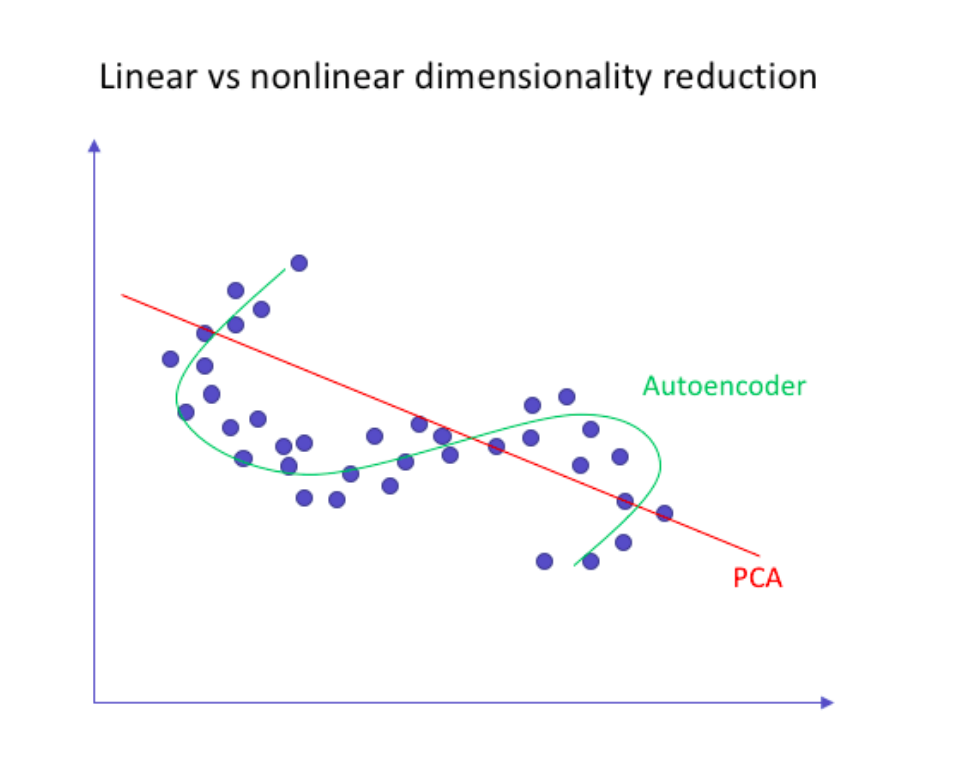
\includegraphics[width=0.70\textwidth]{figs/Autoencoder_non_lineari.png}
	\caption{Differenza fra i metodi lineari (PCA) e gli autoencoder non lineari \cite{Autoencoders}.}
	\label{autoencoder_non_lineari}
\end{figure}


\newpage

%%%%%%%%%%%%%%%%%%%%%%%%%%%%%%%%%%%%%%%%%%%%%%%%%%%%%%%%%%%%%%%%

\subsection{Variational Autoencoders (VAEs)}
\label{VAEs}

Nella sezione precedente è stato presentato l'autoencoder come un metodo di riduzione della dimensionalità; tuttavia, apportando una sostanziale modifica, tale metodo può essere utilizzato per la generazione di eventi ed in questo caso si parla di Variational Autoencoders (VAEs). \\ 
L'autoencoder agisce su di un evento originale $\vec{x}$ trasformandolo in un $\vec{z} = e(\vec{x})$ nello spazio latente (fase di \textbf{encoding}) e poi trasforma nuovamente $\vec{z}$ per tornare allo spazio originale. Per la generazione, basterebbe prendere un punto a caso nello spazio latente, e quindi decodificarlo, ottenendo un nuovo evento non legato direttamente a quello di input, ma solo alla distribuzione nello spazio latente. Questo non tiene pero' conto della regolarità dello spazio latente.\\ 
L'autoencoder codifica in modo puntuale ogni evento associando ad ognuno di essi un punto specifico e diverso dagli altri all'interno dello spazio latente. In questo modo, se viene dato in input un evento mai incontrato durante la fase di addestramento, si presentano delle difficoltà nella sua successiva rigenerazione. In questo caso infatti il modello comincia la fase di rigenerazione a partire da un punto nello spazio latente a cui non è associato nessun input, come se in quel punto lo spazio latente fosse discontinuo (un esempio è riportato in figura \ref{limite autoencoder}). Per ovviare a questo problema, la fase di codifica deve assumere un significato probabilistico, associando ai vari vettori evento non più un solo punto ma un'intera distribuzione. In questo modo lo spazio latente sarà meno soggetto ad avere discontinuità al suo interno, facilitando così il processo di generazione.

\begin{figure}[h!]
	\centering
	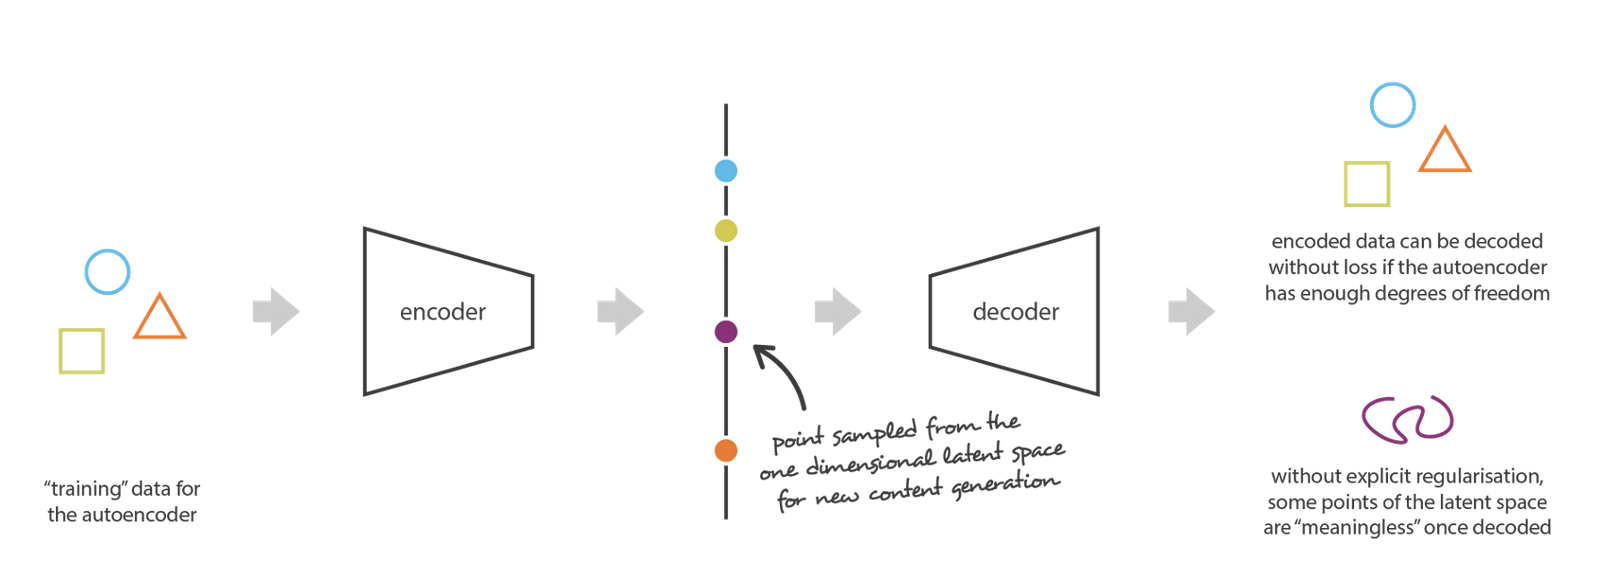
\includegraphics[width=0.99\textwidth]{figs/limite_autoencoder.png}
	\caption{Illustrazione grafica e semplificata dei limiti nell'applicazione degli autoencoder per fini di generazione di nuovi pattern \cite{Understanding_VAEs}.}
	\label{limite autoencoder}
\end{figure}
 

Si può quindi pensare al VAEs come un autoencoder per il quale si attua una regolarizzazione dello spazio latente durante il processo di addestramento ed è quindi adatto alla generazione di nuovi pattern. \\
Lo spazio latente si dice regolare se:
\begin{itemize}
	\item è continuo, ovvero due punti vicini portano ad un risultato simile una volta decodificati;
	\item è completo, nel senso che un qualunque punto porta ad un risultato sensato una volta decodificato.  
\end{itemize}
I VAEs, al pari degli autoencoders, sono costituiti da una coppia di encoder e decoder con la differenza che, per gli autoencoders l'evento di partenza viene codificato come un punto nello spazio latente ($\vec{z}$), mentre per i VAEs la codifica avviene tramite una distribuzione nello spazio latente ($p(\vec{z}|\vec{x})$). Il processo seguito nella fase di addestramento è il seguente:
\begin{enumerate}
	\item L'evento iniziale viene codificato nello spazio latente come una distribuzione di probabilità;
	\item Si campiona un punto dello spazio latente a partire dalla distribuzione del punto precedente;
	\item Tale punto viene decodificato dal decoder, ottenendo un evento ricostruito;
	\item Avviene il confronto fra l'evento iniziale e quello ricostruito da cui si calcola l'errore, che viene poi propagato mediante il meccanismo della \textbf{backpropagation}.
\end{enumerate}

Nella pratica si cerca di fare in modo che la distribuzione ottenuta alla fine del processo di codifica sia il più possibile vicina ad una distribuzione Normale. In particolare si farà in modo che l'encoder restituisca la media e la matrice di covarianza della distribuzione Normale. \\ 
Seguendo questa linea, si ottiene che il processo di addestramento è regolato da una funzione di perdita, composta da un termine relativo alla ricostruzione ed uno relativo alla regolarizzazione dello spazio latente; tale termine di regolarizzazione viene espresso mediante la $\textit{Divergenza di Kullback-Leibler}$, che rappresenta una misura della differenza ta due distribuzioni di probabilità. \\
Il solo fatto di codificare gli eventi di input come delle distribuzioni non garantisce la continuità e la completezza, perché se non si inserisce il termine di regolarizzazione nella funzione di perdita il VAE continuerà a comportarsi come un semplice autoencoder, tendendo semplicemente a minimizzare l'errore di ricostruzione in due possibili modi, cioè codificando gli eventi come distribuzioni da un lato con varianze molto piccole (quasi come singoli punti) e dall'altro con medie molto diverse fra loro (punti molto lontani nello spazio latente); nel primo caso non viene garantita la continuità e nel secondo la completezza. \\ 
Per ottenere la regolarità dello spazio latente si richiede allora che le distribuzioni con cui vengono codificati gli eventi siano il più possibile vicine a distribuzioni Normali con media zero e matrice di covarianza uguale all'identità; le medie saranno allora vicine con conseguente sovrapposizione delle distribuzioni, anche perché la matrice di covarianza così fatta impedisce la codifica come punti nello spazio latente. Il prezzo da pagare sarà un più alto errore nella fase di ricostruzione.\\ \color{red} da chiedere \color{black} \\
Prima di passare alla formulazione matematica dei VAEs, bisogna notare che la regolarità dello spazio latente implica la presenza di un gradiente, il quale permette di mischiare le caratteristiche dei pattern in input e quindi di dare un significato al campionamento nello spazio latente. \\

\color{red}
da chiedere l'ultimo commento
\color{black}

\newpage

%%%%%%%%%%%%%%%%%%%%%%%%%%%%%%%%%%%%%%%%%%%%%%%%%%%%%%%%%%%%%%%
\subsubsection{Formulazione matematica dei VAEs}
\label{matematica dei VAEs}

Per formulare in maniera rigorosa i VAEs è necessario utilizzare l' inferenza variazionale e verranno dati alcuni concetti fondamentali della teoria dell'informazione. \\
La quantità di informazione in una preposizione (nel nostro caso l'evento) è definita come:
\begin{equation}
	I = \log p(x)
\end{equation}
dove x è l'evento. \\
Quindi ad eventi certi o molto probabili corrisponde una quantità di informazione nulla o molto bassa, mentre ad eventi poco probabili corrisponde una quantità di informazione più alta. \\ 
Un'altra quantità fondamentale nella teoria dell'informazione è l'\textit{entropia}, ovvero l'informazione media, ed è definita nel seguente modo:
\begin{equation}
	H = \sum p(x) \log p(x)
\end{equation}
La divergenza di KL è la misura di dissimilarità tra due distribuzioni (p(x) e q(x)):
\begin{equation}
	KL(p(x)||q(x)) = -\sum p(x) \log q(x) + \sum p(x) \log p(x) = -\sum p(x) \log \frac{q(x)}{p(x)}
\end{equation}
e si nota come essa sia molto simile alla differenza delle entropie delle due distribuzioni perché due distribuzioni che hanno un'informazione media uguale saranno pressoché uguali.
Le due proprietà fondamentale della \textit{KL divergency} sono le seguenti:
\begin{enumerate}
	\item 
	\begin{equation}
		KL(p(x)||q(x)) \geq 0
	\end{equation}
	
	\item 
	\begin{equation}
		KL(p(x)||q(x)) \not = KL(q(x)||p(x))
	\end{equation}
\end{enumerate}
cioè la divergenza di KL è semi-definita positiva e non è simmetrica. \\
Ora è possibile ricollegarsi al discorso sui VAEs e si definisca con $\vec{x}$ la grandezza osservabile e con $\vec{z}$ quella nascosta dello spazio latente. Il teorema di Bayes \cite{Statistica} permette di scrivere:
\begin{equation}
	p(\vec{z}|\vec{x}) = \frac{p(\vec{x}|\vec{z}) p(\vec{z})}{p(\vec{x})}
	\label{bayes}
\end{equation}
dove
\begin{equation}
	p(\vec{x}) = \int p(\vec{x}|\vec{z}) p(\vec{z}) dz
	\label{integrale}
\end{equation}
tuttavia tale integrale è difficile da calcolare e quindi è possibile approssimare $p(\vec{z}|\vec{x})$ con $q(\vec{z}|\vec{x})$ utilizzando l'inferenza variazionale. Si assume inoltre che quest'ultima debba essere scelta dalla famiglia delle distribuzioni Normali, andando a variare i parametri in modo che risulti il più possibile simile a $p(\vec{z}|\vec{x})$, che viene detta \textit{prior} e rappresenta la scelta a priori per la modellizzazione dello spazio latente; generalmente viene scelta una distribuzione normale multivariata standard e la $q(\vec{z}|\vec{x})$ deve approssimare tale distribuzione durante la fase di addestramento. Per vincolare la forma di $q(\vec{z}|\vec{x})$ a quella di $p(\vec{z}|\vec{x})$ viene utilizzata la \textbf{KL divergency}: 


\begin{equation}
	KL (q(\vec{z}|\vec{x}) || p(\vec{z}|\vec{x})) = -\sum q(\vec{z}|\vec{x}) \log \frac{p(\vec{z}|\vec{x})}{q(\vec{z}|\vec{x})}
\end{equation}

e sostituendo $p(\vec{z}|\vec{x})$ con la~\ref{bayes} si ottiene:


\begin{align*} 
	KL (q(\vec{z}|\vec{x}) || p(\vec{z}|\vec{x})) &=  -\sum q(\vec{z}|\vec{x}) \log \frac{p(\vec{x}|\vec{z})p(\vec{z})}{p(\vec{x})q(\textbf{z}|\vec{x})} \\ &=  -\sum q(\vec{z}|\vec{x})\log \frac{p(\vec{x}|\vec{z})p(\vec{z})}{q(\vec{z}|\vec{x})} + \sum q(\vec{z}|\vec{x})\log p(\vec{x})
\end{align*}
ma in entrambi i termini della somma la sommatoria è estesa sulle z, quindi:

\begin{align*}
	\sum q(\vec{z}|\vec{x})\log p(\vec{x}) =
	\log (\vec{x}) \sum q(\vec{z}|\vec{x}) =
	\log p(\vec{x})
\end{align*}
perché $\sum q(\vec{z}|\vec{x})=1$. \\
Si arriva quindi al seguente risultato:
\begin{equation}
	\log p(\vec{x}) = KL (q(\vec{z}|\vec{x}) || p(\vec{z}|\vec{x})) + \sum q(\vec{z}|\vec{x}) \log \frac{p(\vec{x}|\vec{z})p(\vec{z})}{q(\vec{z}|\vec{x})}
	\label{introL}
\end{equation}
La sommatoria nell'equazione~\ref{introL} prende il nome di $\textit{Variational lower bound}$ e viene indicata con la lettera $\mathcal{L}$. \\
A questo punto si deve osservare che $\vec{x}$ è fissato e quindi il termine sinistro dell'equazione \ref{introL} è una costante; di conseguenza minimizzare la $\textbf{KL divergency}$ equivale a massimizzare la $\mathcal{L}$, che può essere riscritta in maniera semplificata:

\begin{equation}
\label{eq:lower_bound}
\begin{split}
	\mathcal{L} &= \sum q(\vec{z}|\vec{x}) \log \frac{p(\vec{x}|\vec{z})p(\vec{z})}{q(\vec{z}|\vec{x})} \\
	 &=\sum q(\vec{z}|\vec{x}) \log p(\vec{x}|\vec{z}) + \sum q(\vec{z}|\vec{x}) \log \frac{p(\vec{z})}{q(\vec{z}|\vec{x})} \\
	  &= E_{q}\log p(\vec{x}|\vec{z}) - KL (q(\vec{z}|\vec{x}) || p(\vec{z}))
\end{split}
\end{equation}

Quindi l'obiettivo è quello di trovare la distribuzione $p(\vec{z}|\vec{x})$ che è troppo complessa per essere calcolata in modo analitico: si cerca di approssimarla con una $q(\vec{z}|\vec{x})$ scelta tra un'opportuna famiglia e, per scegliere quella più vicina, si deve minimizzare $KL (q(\vec{z}|\vec{x}) || p(\vec{z}|\vec{x}))$, che come visto equivale a massimizzare la $\mathcal{L}$. \\
In figura \ref{grafo} è possibile osservare in che modo si passa da $\vec{x}$ a $\vec{z}$ e viceversa.

\newpage

\begin{figure}[h!]
	\centering		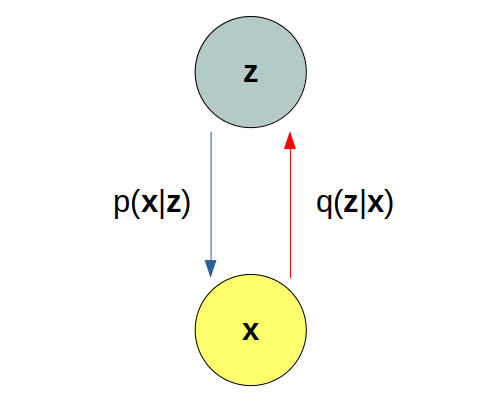
\includegraphics[width=0.40\textwidth]{figs/grafoVAE.png}
	\caption{Illustrazione grafica della modalità attraverso la quale si ottiene il passaggio dalla variabile $\vec{x}$ osservabile alla $\vec{z}$ nello spazio latente e viceversa.}
	\label{grafo}
\end{figure}

Il significato del termine di $\textbf{KL divergency}$ che compare in $\mathcal{L}$ suggerisce che la distribuzione $q(\vec{z}|\vec{x})$ debba essere il più possibile simile ad una distribuzione $p(\vec{z})$ che può essere scelta e quindi si assume una distribuzione Normale multivariata standard, per la quale la KL divergency è più facile da calcolare. \\
L'altro termine in $\mathcal{L}$ è riconducibile ad un errore di ricostruzione, infatti il processo di decodifica, una volta campionato $\vec{z}$ è deterministico e quindi si ottiene che:
\begin{equation}
	p(\vec{x}|\vec{z}) = p(\vec{x}|\hat{\vec{x}})
\end{equation}
dove $\hat{\vec{x}}$ è l'evento ricostruito. Inoltre se si considerano distribuzioni gaussiane si troverà che:

\begin{equation}
	p(\vec{x}|\hat{\vec{x}}) \propto e^{{-{\lvert \vec{x}-\hat{\vec{x}}} \rvert}^2}
\end{equation}

e quindi

\begin{equation}
	\log p(\vec{x}|\hat{\vec{x}}) \propto -{\lvert \vec{x}-\hat{\vec{x}} \rvert}^2
\end{equation}

Quindi si osserva che l'autoencoder tende a minimizzare semplicemente ${\lvert \vec{x}-\hat{\vec{x}} \rvert}^2$, mentre il VAE tende a minimizzare la seguente quantità:

\begin{equation}
	{\lvert \vec{x}-\hat{\vec{x}} \rvert}^2 + KL (q(\vec{z}|\vec{x})||N(\vec{\mu},\vec{\Sigma}))
\end{equation}

Nella pratica si costruisce la rete neurale che si occupa della fase di codifica in modo che restituisca i parametri della distribuzione Normale e quindi la media e la matrice di covarianza, che si impone essere diagonale per semplicità; da qui viene campionato un punto dello spazio latente a partire da tale distribuzione e avviato verso il decoder per ottenere l'evento ricostruito da confrontare con quello iniziale (nella fase di addestramento). Lo schema di questo processo è riportato in figura \ref{schemaVAEs}.
\newpage

\begin{figure}[h!]
	\centering		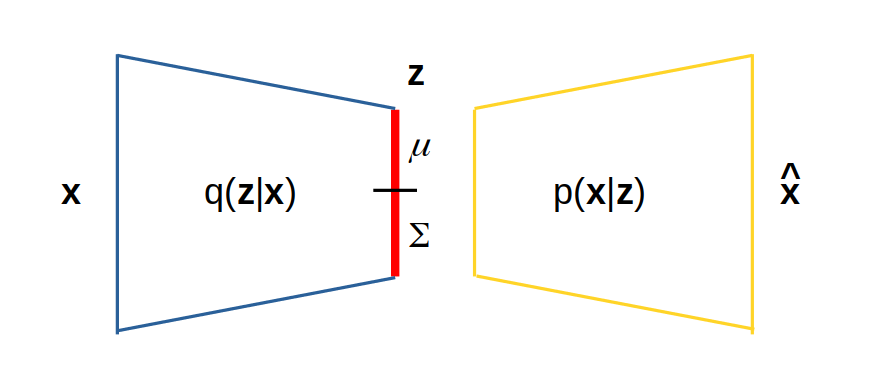
\includegraphics[width=0.80\textwidth]{figs/VAEgauss.png}
	\caption{Schema di funzionamento del VAE, dove viene messo in evidenza che l'encoder è forzato a restituire come output i parametri della distribuzione Normale, ovvero la media e la matrice di covarianza.}
	\label{schemaVAEs}
\end{figure}


Infine, per la fase di generazione di nuovi eventi, sarà sufficiente eliminare l'encoder e campionare dalla distribuzione che si è ottenuta alla fine dell'addestramento e fornire tale punto al decoder per costruire un nuovo evento.

\color{red}
commento: cosa significano le proprietà della KL divergency ?
\color{black}

\newpage